\documentclass[a4paper,12pt]{article}
% \documentclass[a4paper,12pt,draft]{article}

\usepackage[T1,T2A]{fontenc}
\usepackage[utf8]{inputenc}
\usepackage[english,russian]{babel}

\usepackage[left=30mm,right=15mm,
    top=20mm,bottom=20mm,bindingoffset=0cm]{geometry}
\parindent 11mm

\usepackage{floatrow}
\floatsetup[table]{style=Plaintop}
\usepackage[labelsep=period]{caption}

\usepackage{setspace}

\usepackage[shortcuts]{extdash}

\usepackage{enumitem}
\setlist[itemize,enumerate]{before={\vspace{-\parsep}},after={\vspace{-\parsep}},itemsep=-0.75\parsep}
\setlist[enumerate,2]{before={\vspace{-2\parsep}},after={\vspace{-2\parsep}},itemsep=-0.75\parsep}
\setlist[itemize,2]{label=$\vartriangleright$,before={\vspace{-2\parsep}},after={\vspace{-2\parsep}},itemsep=-0.75\parsep}

\usepackage{amsmath}
\usepackage{amssymb}
\usepackage{cite}
\usepackage{graphicx}
\usepackage{tikz}
\usepackage[suffix=]{epstopdf}  
\usepackage[unicode, pdftex]{hyperref}

\usepackage{icomma}
\usepackage{multirow}
\usepackage{indentfirst}
\usepackage{tabularx}

\title{DataMatrix}
\author{LeonarD DE}
\date{May 2024}

\newcounter{def}
\newcommand{\newdef}[1]{\addtocounter{def}{1}{\bf Определение \arabic{def}.} #1 \par}
\newcommand{\newdefnp}[1]{\addtocounter{def}{1}{\bf Определение} #1 \par}


\newtheorem{definit}{Определение}

\title{Диплом}
\author{LeonarD DE}
\date{April 2024}

\begin{document}

%========================================================
% титульная страница

\begin{titlepage}

\begin{center}
\MakeUppercase{министерство науки и высшего образования Российской Федерации} 

федеральное государственное автономное образовательное учреждение высшего образования

\MakeUppercase{уральский федеральный университет} 

имени первого Президента России Б.Н. Ельцина
\end{center}

\vspace{5mm}

\begin{center}    
  \MakeUppercase{институт естественных наук и математики} 
\end{center}

\vspace{20mm}

\begin{center}
  Департамент математики, механики и компьютерных наук
\end{center}

\vspace{10mm}

\begin{center}
    \bfseries \MakeUppercase{Разработка программного комплекса моделирования и визуализации движения беспилотных летательных аппаратовы}
\end{center}

\vspace{5mm}

\begin{center}
    Направление подготовки 01.03.01 «Математика»
\end{center}

\vspace{20mm}

\newcolumntype{I}{!{\vrule width 3pt}}
\newlength\savedwidth

\newcommand\whline[1]{%
  \noalign{%
    \global\savedwidth\arrayrulewidth\global\arrayrulewidth 1.5pt%
  }%
  \cline{#1}%
  \noalign{\vskip\arrayrulewidth}%
  \noalign{\global\arrayrulewidth\savedwidth}%
}

\begin{table}[h]
    \centering 
    \begin{tabular}[t]{p{5.5cm} p{1cm} c}
        Директор департамента && Выпускная квалификационная\\ 
         к.ф.-м.н., Е. С. Пьяньзина  &&работа бакалавра\\ 
        %к.ф.-м.н., Е. С. Пьяньзина & \\
        &&\bfseries{Дербенева } \\
        && \bfseries{Леонида Олеговича}\\
        && \\ 
        && \\ \whline{1-1} \cline{3-3}
        && \\ 
        Нормоконтролер: && Научный руководитель:  \\
        О.А. Суслова    && к.ф.-м.н., С.С. Кумков \\ 
        && \\
        && \\ \cline{1-1} \cline{3-3}
        
    \end{tabular}
\end{table}
\vspace{25mm}
\begin{center}
Екатеринбург 

2024
\end{center}

\end{titlepage}


%========================================================
% Реферат
\newpage

\thispagestyle{empty}

\begin{center}
  \textbf{РЕФЕРАТ}  	
\end{center}

\vspace{4mm}

\noindent
Дербенев Л. О.: РАЗРАБОТКА ПРОГРАММНОГО КОМПЛЕКСА МОДЕЛИРОВАНИЯ И ВИЗУАЛИЗАЦИИ ДВИЖЕНИЯ БЕСПИЛОТНЫХ ЛЕТАТЕЛЬНЫХ АППАРАТОВ, Выпускная квалификационная работа на соискание степени бакалавра по направлению подготовки 01.03.01 <<Математика>>, \pageref{LastPage}~с., рис.~???, источн.~???.

\bigskip

{\raggedright
\noindent
Ключевые слова: БЕСПИЛОТНЫЕ ЛЕТАТЕЛЬНЫЕ АППАРАТЫ, АВТОМАТИЧЕСКОЕ РАЗРЕШЕНИЕ КОНФЛИКТНЫХ СИТУАЦИЙ, РАЗРЕШАЮЩИЕ МАНЕВРЫ, МОДЕЛИРОВАНИЕ ДВИЖЕНИЯ БПЛА, МОДЕЛИ ДИНАМИКИ

}

\bigskip

\noindent
В настоящее время активно развивается движение гражданских беспилотных летательных аппаратов (БПЛА). При этом возникают конфликты БПЛА с другими БПЛА, а также с самолётами малой авиации и вертолётами, которые движутся в тех же районах и на тех же высотах, что и БПЛА. В таких условиях важной является разработка алгоритмов для бортовых компьютеров БПЛА для автоматической выработки и отработки манёвров, разрешающих возникающие конфликтные ситуации с другими летательными аппаратами. В работе описывается разработка программного комплекса для моделирования движения БПЛА и процесса разрешения конфликтных ситуаций, позволяющей оценивать качество тех или иных процедур выработки разрешающего маневра. Вычислительный комплекс разработан на языке C++. Также с использованием библиотеки Plotly.PY на языке Python создана программа постериорной визуализации результатов моделирования для визуального контроля движения БПЛА и принимаемых решений. 
  

%========================================================
% Содержание
\newpage
\setcounter{page}{2}
\tableofcontents
\newpage

%========================================================
% Введение
\newpage
\section*{Введение}
\addcontentsline{toc}{section}{Введение}

В настоящее время активно развивается движение гражданских беспилотных летательных аппаратов (БПЛА). С их помощью проводится доставка различных грузов в удаленные поселки (чем раньше занималась только малая авиация), мониторинг состояния природных и искусственных объектов (лесов, озер, рек, трубо-, нефте- и газопроводов, ЛЭП и др.).

При этом конфликтов БПЛА и больших самолётов почти не возникает: в рабочем режиме они движутся на разных высотах, а вход БПЛА в аэропортовые зоны весьма жёстко регламентируется. Однако возникают конфликты БПЛА  с другими БПЛА, а также с самолётами малой авиации и вертолётами, которые движутся в тех же районах и на тех же высотах, что и БПЛА. 

Ситуация такова, что движение БПЛА не диспетчеризируется централизовано, как движение больших самолётов. Часто полет малого ЛА объявляется в уведомительном порядке. Поэтому текущая воздушная обстановка актуально недоступна операторам БПЛА, которые, кроме того, не имеют связи между собой и с диспетчерскими службами УВД. В то же время достаточно чётко прописаны регламенты того, какую информацию о собственном движении во время полёта БПЛА сообщает в эфир в виде широковещательных пакетов.

В таких условиях важной является разработка алгоритмов для бортовых компьютеров БПЛА для обработки полученной информации о движении окружающих летательных аппаратов, малых и больших, и для последующей автоматической выработки и отработки манёвров, разрешающих возникающие конфликтные ситуации с другими летательными аппаратами. 

В рамках создания таких алгоритмов важным является численное моделирование ансамбля БПЛА, движущихся по тем или иным траекториям в тех или иных условиях. Такое моделирование позволяет провести предварительную оценку качества предлагаемых манёвров, разрешающих конфликты. Для адекватности проводимых оценок требуется, чтобы модели движения и маневрирования БПЛА достаточно точно соответствовали движению реальных аппаратов. 

В рамках данной работы были предприняты шаги в направлении создания такого моделирующего программного комплекса, включающего реализации основных моделей движения БПЛА, модели радиообменов и процедур обнаружения конфликтов. В дальнейшем в этот комплекс можно встраивать и тестировать те или иные алгоритмы выработки манёвров уклонения с целью оценки их качества.

%========================================================
% Основная часть
\newpage

\section{Постановка задачи}

Входной информацией для моделирующего комплекса является набор данных о каждом БПЛА из рассматриваемого ансамбля. Сюда входит информация о типе динамики данного БПЛА, её параметрах, а также априорный полетный план. Описание плана представляет собой номинальную траекторию движения, представляющую собой ломаную линию в пространстве, описываемую координатами своих вершин и моментами времени, когда планируется проход БПЛА через них.

Модели динамики жестко прописываются в коде комплекса и включают в себя модели, представляющих движение аппаратов самолетного, вертолетного типа и коптеров. Параметры модели динамики задаются индивидуально для каждого БПЛА.

Движение на промежутках между парами последовательных точек предполагается равномерным прямолинейным, так что положения точек и времена их прохода определяют скорость движения на каждом промежутке. 

Для моделирования движения каждого БПЛА требуется реализовать процедуру углового разворота, адекватную для каждого типа динамики. Данная процедура вырабатывает движение БПЛА вблизи контрольных точек маршрута, <<срезающее>> угол ломаной (что отражает реальное движение БПЛА в такой ситуации). Здесь планируется вырабатывать некоторое разумное движение~--- \textit{штурманскую прокладку}, сопрягающее два соседних отрезка планового маршрута и скорости движения на каждом из них. Выработка управления БПЛА на участках углового разворота производится посредством ПИД\=/регулятора, прицеливающего на штурманскую прокладку.

Для блока моделирования радиообменов предусматривается выработка информации, вещаемой в эфир каждым БПЛА при реальном движении. Для комплекса существенными являются два типа информационных пакетов: с текущем положением БПЛА и с краткосрочным прогнозом его движения. Такая информация необходима для выявления конфликтных ситуаций между БПЛА и выработки разрешающих маневров.

Кроме того, в комплекс требуется передавать параметры интегрирования движения БПЛА: шаг интегрирования, шаг записи информации о положении БПЛА в выходной файл.

На выходе комплекс должен выдавать в файл информацию о результатах моделирования движения каждого БПЛА и о процессах принятия решения, происходящих на борту:
\begin{itemize}
  \item начальный полетный план;
  \item изменения полетного плана вследствие выработки маневров, разрешающих конфликты;
  \item набор положений БПЛА в моменты с заданной сетки по времени (для визуализации);
  \item пакеты вещания (с текущими положениями БПЛА и краткосрочными прогнозами движения);
  \item индикация наличия конфликтов.
\end{itemize}

\newpage



\section{Теоретическая часть}

\subsection{Рассматриваемые модели динамики}

Считается, что выбрана стандартная система координат, используемая в системах УВД: начало координат~$O$ выбрано где-то в районе управления, ось $Ox$ направлена на восток, ось $Oz$~--- на сервер, ось $Oy$ направлена вертикально вверх. Таким образом, движение по оси~$y$ является вертикальным движением и часто описывается отдельно от движения в плоскости~$Oxz$.


\subsubsection{Материальная точка}

Материальная точка --- это идеализированное тело, обладающее массой, но не имеющее размеров. В физике материальная точка используется как модель для описания движения объекта, когда его размерами можно пренебречь по сравнению с масштабами задачи. В рамках создаваемого комплекса данная модель является вспомогательной, используемой при отладке, поскольку, в частности, движения соответствующего объекта достаточно просто понимаемы.

Материальная точка имеет следующую модель движения:
\begin{equation}
    \Ddot{r} = m \cdot u,
\end{equation}
где $r = (x, y, z)^\text{\textup{T}}$~--- радиус\=/вектор положения объекта, $u = (u_x, u_y, u_z)^\text{\textup{T}}$~--- управление, являющееся ускорением, $m$~--- масса точки. Является параметром системы.

Покоординатная запись:
\begin{equation*}
  \ddot{x} = u_x, \quad \ddot{y} = u_y, \quad \ddot{z} = u_z.
\end{equation*}

Запись, включающая скорости:
\begin{alignat*}{3}
  & \dot{x} = V_x,  & \quad & \dot{y} = V_y, & \quad & \dot{z} = V_z, \\
  & \dot{V_x} = u_x, & & \dot{V_y} = u_y, & & \dot{V_z} = u_z.
\end{alignat*}

На управление накладывается геометрическое ограничение $\|u\| \leqslant u^{\max}$. Также возможен вариант ограничений, развязывающий горизонтальное и вертикальное движение: $\big\|(u_x,u_z)\big\| \leqslant u^{\max}_\text{гор}$, $|u_y| \leqslant u^{\max}_\text{верт}$.


\subsubsection{Коптер}  

Недостаток модели материальной точки заключается в том, что нет никаких ограничений на максимальную скорость, развиваемую объектом, а также отсутствие учета сопротивления среды (воздуха) движению объекта.

Простейшей моделью, учитывающей эти обстоятельства, является модель, управляемая \textit{командным сигналом} скорости:
\begin{alignat*}{3}
  & \dot{x} = V_x, & \quad & \dot{y} = V_y, & \quad
    & \dot{z} = V_z, \\
  & \displaystyle
    \dot{V_x} = \frac{u_x - V_x}{l_{xz}},  & &
    \dot{V_y} = \frac{u_y - V_y}{l_{y}},   & &
    \dot{V_z} = \frac{u_z - V_y}{l_{xz}}.
\end{alignat*}
Здесь $u = (u_x, u_y, u_z)^\text{\textup{T}}$~--- управление, командный сигнал скорости, имеющий смысл желаемой скорости по каждой из координат; $l_{xz}$, $l_y$~--- коэффициенты, описывающие инерционность выхода на выбранный уровень скорости: выход осуществляется за время порядка $3l$. 

Командный сигнал ограничен по модулю, что соответствует максимально возможной скорости, которую может развивать ЛА. 

Данная модель является простейшей моделью движения лёгкого коптера, который достаточно быстро может менять скорость своего движения, но имеет ограничение по максимальной скорости из-за относительно малой мощности двигателя. 

\subsubsection{Вертолетная модель}

Величины вертикальной и горизонтальной скоростей коптера обусловлены, по большому счету, только скоростью вращения винтов коптера. Направление горизонтальной скорости и соотношение горизонтальной и вертикальной скоростей обусловлены углом наклона коптера. И то, и другое достаточно быстро меняется.

В случае с достаточно большим БПЛА вертолетного типа изменение угловой ориентации уже достаточно ощутимо длительный процесс, так что в модели вертолетной динамики следует развязать управление величинами вертикальной и горизонтальной скоростей, а также управление курсом движения аппарата:
\begin{equation*}
  \begin{array}{l}
    \dot x = V_\text{гор} \cos \psi, \\[0.75ex]
    \dot z = V_\text{гор} \sin \psi, \\[0.75ex]
    \dot y = V_\text{верт}, \\[0.75ex]
    \dot \psi   = \frac{\beta_\text{бок}}{V_\text{гор}} \, u_\text{бок}, \quad |u_\text{бок}| \leqslant 1, \\[0.75ex]
    \dot V_\text{гор} = a, \quad  
      a_{\min} \leqslant a \leqslant a_{\max},
      \quad V^{\min}_\text{гор} \leqslant V_\text{гор} \leqslant V^{\min}_\text{гор}, \\[0.75ex]
    \dot V_\text{верт} = u_\text{верт},
      \quad u^{\min}_\text{верт} \leqslant u_\text{верт} \leqslant u^{\max}_\text{верт}, \quad
      V^{\min}_\text{верт} \leqslant V_\text{верт} \leqslant V^{\max}_\text{верт}.
  \end{array}
\end{equation*}

Здесь $\psi$~--- угол курса; $u_\text{бок}$~--- ускорение, управляющее разворотом круса; $u_\text{верт}$~--- ускорение (создаваемое изменением скорости вращения винтов), управляющее вертикальной скоростью; $a$~--- ускорение, управляющее величиной горизонтальной скорости (продольное); $\beta_\text{бок}$~--- коэффициент горизонтальной маневренности судна.

Динамика для изменение курсового угла использует традиционное описание со скоростью в знаменателе: чем выше скорость, тем ниже маневренность аппарата, то есть тем медленнее меняет аппарат направление движения при тех же боковых ускорениях.

Заметим, что сама по себе модель не включает ограничения на величины скоростей, их приходится ограничивать через дополнительно вводимые неравенства. Можно подменить управление скоростью через ускорение на управление скоростью через командный сигнал, что даст ограничение на максимальные скорости в виде ограничения на максимальное значение соответствующего командного сигнала:
\begin{equation*}
  \begin{array}{l}
    \dot x = V_\text{гор} \cos \psi, \\[0.75ex]
    \dot z = V_\text{гор} \sin \psi, \\[0.75ex]
    \dot y = V_\text{верт}, \\[0.75ex]
    \dot \psi   = \frac{\beta_\text{бок}}{V_\text{гор}} \, u_\text{бок}, \quad |u_\text{бок}| \leqslant 1, \\[0.75ex]
    \dot V_\text{гор} = (V^\text{упр}_\text{гор} - V_\text{гор}) / l_\text{гор}, \quad  
      V^{\text{упр},\min}_\text{гор} \leqslant V^\text{упр}_\text{гор} \leqslant V^{\text{упр},\max}_\text{гор}, \\[0.75ex]
    \dot V_\text{верт} = (V^\text{упр}_\text{верт} - V_\text{верт}) / l_\text{верт}, \quad  
      V^{\text{упр},\min}_\text{верт} \leqslant V^\text{упр}_\text{верт} \leqslant V^{\text{упр},\max}_\text{верт}.
  \end{array}
\end{equation*}


\subsubsection{Самолетная модель}

При движении самолета его вертикальная скорость обусловлена \textit{углом атаки}~--- углом между плоскостью крыла и скоростью набегающего потока. Угол плоскости крыла связан с \textit{углом тангажа}, то есть с углом наклона самолета относительно оси, проходящей через плоскость крыла перпендикулярно фюзеляжу. Таким образом, управление движением самолета связано с управлением не только углом курса, но и углом тангажа:
\begin{equation*}
  \begin{array}{l}
    \dot x = V \cos \theta \cos \psi, \\[0.75ex]
    \dot z = V \cos \theta \sin \psi, \\[0.75ex]
    \dot y = V \sin \theta, \\[0.75ex]
    \dot \theta = \frac{\beta_\text{верт}}{V} \, u_\text{верт}, \\[0.75ex]
    \dot \psi   = \frac{\beta_\text{бок}}{V} \, u_\text{бок}, \\[0.75ex]
    |u_\text{верт}| \leqslant 1, 
      \quad |u_\text{бок}| \leqslant 1, \\[0.75ex]
    \dot V = a, \quad  
      a_{\min} \leqslant a \leqslant a_{\max},
      \quad V_{\min} \leqslant V \leqslant V_{\max}.
  \end{array}
\end{equation*}

Здесь $\theta$~--- угол тангажа, $\psi$~--- угол курса; $u_\text{верт}$, $u_\text{бок}$~--- ускорения, управляющие углами тангажа и курса; $a$~--- ускорение, управляющее скоростью; $\beta_\text{верт}$, $\beta_\text{бок}$~--- коэффициенты маневренности судна. Модель взята из~\cite{bib:GOST}.

Заметим, что скорость уже имеет единое значение, поскольку именно величина линейной скорости вкупе с текущей угловой ориентацией обуславливает вертикальную и горизонтальную составляющую скорости аппарата.

Опять, управление скоростью через ускорения можно заменить на управление через командный сигнал и отказаться от ограничений на величину скорости:
\begin{equation*}
  \begin{array}{l}
    \dot x = V \cos \theta \cos \psi, \\[0.75ex]
    \dot z = V \cos \theta \sin \psi, \\[0.75ex]
    \dot y = V \sin \theta, \\[0.75ex]
    \dot \theta = \frac{\beta_\text{верт}}{V} \, u_\text{верт}, \\[0.75ex]
    \dot \psi   = \frac{\beta_\text{бок}}{V} \, u_\text{бок}, \\[0.75ex]
    |u_\text{верт}| \leqslant 1, 
      \quad |u_\text{бок}| \leqslant 1, \\[0.75ex]
    \dot V = (V^\text{упр} - V) / l, \quad  
      V^\text{упр}_{\min} \leqslant V^\text{упр} \leqslant V^\text{упр}_{\max}.
  \end{array}
\end{equation*}


\subsection{Полетный план}

В начале движения БПЛА имеет свой полетный план, задаваемый как совокупность $\{(r_i, t_i)\}_{i=1}^n$, где $r_i=(x_i,y_i,z_i)$~--- точка трехмерного пространства, $t_i$~--- момент времени, в который БПЛА должен оказаться в заданной точке. Считаем, что $t_i < t_{i+1}$.

Считается, что между соседними точками полетного плана БПЛА движется равномерно прямолинейно, так что на отрезке $[r_i,r_{i+1}]$ его скорость находится как
$$
  V_i = \frac{r_{i+1} - r_i}{t_{i+1} - t_i}\,.
$$

\subsection{Построение штурманской прокладки}

Заметим, что заданная траектория является ломаной линией. Однако БПЛА в точках излома не может мгновенно менять направление скорости. Как следствие встает вопрос о том, как 

???????????

Пусть $n>1$, рассмотрим отрезок пути $(r_k,t_k)$, $(r_{k+1},t_{k+1})$, $k=1\dots n-1$. По определению, летательный аппарат должен оказаться в точке $r_k$ в момент времени $t_k$ и в точке $r_{k+1}$ в момент $t_{k+1}$. Или другими словами БПЛА должен пройти расстояние $S_k= |r_{k+1} - r_{k}|$ за время $\tau_i = t_{k+1} - t_{k}$. Значит мы можем найти скорость $V_k = \frac{S_k}{\tau_k}$.

Пусть теперь $n>2$, рассмотрим два отрезка, заданные тремя точками $(r_k,t_k)$, $(r_{k+1},t_{k+1})$, $(r_{k+2},t_{k+2})$ $k=1\dots n-2$. Найдем для скорости $V_k$ и $V_{k+1}$ для них, как это было сделано выше. Другими словами, наш БПЛА должен моментально сменить скорость в точке $(r_{k+1},t_{k+1})$ с $V_k$ на $V_{k+1}$, но в реальной жизни летательные аппараты так не могут. Данную проблемы решает \textit{штурманская прокладка}, она позволит плавно переходить с одного отрезка на другой и также плавно менять скорость. По сути аппарат будет прицеливаться на нее. О ее построении будет пункт чуть ниже.

???
И какие-то слова о том, что под углом летать не умеем~--- надо прокладку и прицеливаться на нее

\subsection{ПИД-регулятор}
ПИД-регулятор (пропорционально\=/интегрально\=/дифференциальный регулятор) является одним из наиболее распространенных методов регулирования систем управления. Он состоит из трех основных компонентов: пропорциональной, интегральной и дифференциальной составляющих.

Пропорциональная составляющая определяет выходной сигнал контроллера пропорционально разности между желаемым и текущим значением управляемой величины. Это позволяет реагировать на ошибку управления и регулировать систему.

Интегральная составляющая интегрирует ошибку управления с течением времени, что позволяет уменьшить статическую ошибку системы и обеспечить точное следование заданному значению.

Дифференциальная составляющая учитывает скорость изменения ошибок и предотвращает быстрые колебания системы, обеспечивая более плавное и стабильное управление.

В итоге, комбинация трех компонентов ПИД-регулятора позволяет эффективно и точно управлять системой, обеспечивая минимальное перерегулирование и быстрое достижение заданного значения.

Пусть $r$~--- заданное значение, которое нужно поддерживать, $e = (r-y)$ - невязка или ошибка регулирования. Тогда для линейной, стационарной системы ПИД-регулятор имеет вид:
\begin{equation}
    u(t) = P + I + D = K_p\cdot e(t) + K_i \cdot \int\limits_0^\text{\textup{T}} e(t) d\tau + K_d \frac{de}{dt},
\end{equation} 
где $K_p$, $K_i$, $K_d$~--- коэффициенты усиления пропорциональной, интегрирующей и дифференцирующей составляющих.

Рассмотрим простую линейную задачу:
\begin{equation}\label{PID}
    \Dot{x} = Ax + Bu,\quad x \in R^n, u \in R^m
\end{equation}

$u = 0 $~--- разрешенное управление. Отсюда следует, что $x = 0$ является точкой равновесия. Задача вывести систему в точку равновесия.

В данной работе был использован линейный пропорциональный регулятор, то есть $u = Kx$, где $K~\in~R^{m\times n}$.
Теперь задача имеет вид:
\begin{equation}\label{PID_lin}
    \Dot{x} = Ax + BKx = (A+BK)x
\end{equation}

Данная система является устойчивой $\Longleftrightarrow$ $\forall \lambda$~--- собственное значение, выполняется: $Re\lambda < 0$.

В данной работе будем использовать только пропорциональный регулятор:

$$u = -k_x \cdot (x - x_w) - k_V\cdot (V_x - V_{x,w})$$


\subsection{Построение регулятора для материальной точки}

Построим регулятор для материальной точки. Мы имеем
\begin{equation*}
    \Ddot{r} = u
\end{equation*}
или распишем в эквивалентной форме
\begin{align*}
    \ddot{x} = u_x \\
    \ddot{y} = u_y \\
    \ddot{z} = u_z
\end{align*}
Пусть $X = (x,y,z,v_x,v_y,v_z)^\text{\textup{T}}$, где $v_i$~--- соответствующие компоненты скорости.

Запишем задачу:
\begin{align*}
    \Dot{X} = AX + Bu =
            \begin{pmatrix}
                0& 0& 0& 1& 0& 0\\
                0& 0& 0& 0& 1& 0\\
                0& 0& 0& 0& 0& 1\\
                0& 0& 0& 0& 0& 0\\
                0& 0& 0& 0& 0& 0\\
                0& 0& 0& 0& 0& 0\\
            \end{pmatrix} 
            \cdot X +
            \begin{pmatrix}
                0& 0& 0\\
                0& 0& 0\\
                0& 0& 0\\
                1& 0& 0\\
                0& 1& 0\\
                0& 0& 1\\
            \end{pmatrix}
            \cdot u = 
            &\begin{pmatrix}
                O_3& I_3\\
                O_3& O_3\\ 
            \end{pmatrix}
            \cdot X +
            \begin{pmatrix}
                O_3\\
                I_3\\
            \end{pmatrix}
            \cdot u
\end{align*}
То есть можно сказать, что $K\in R^{3\times 6}$ или другими словами у нас 18 параметров, но заметим, что так как мы используем пропорциональный регулятор, то не равны нулю лишь $K_{x\rightarrow u_x}$, $K_{y\rightarrow u_y}$, $K_{z\rightarrow u_z}$, $K_{v_x\rightarrow u_x}$, $K_{v_y\rightarrow u_y}$, $K_{v_z\rightarrow u_z}$:

\begin{align*}
K =
\begin{pmatrix}
    K_{x\rightarrow u_x}& 0& 0& K_{v_x\rightarrow u_x} & 0& 0\\
    0& K_{y\rightarrow u_y} & 0& 0& K_{v_y\rightarrow u_y} & 0\\
    0& 0& K_{z\rightarrow u_z} & 0& 0& K_{v_z\rightarrow u_z} \\
\end{pmatrix}
\end{align*}

То есть получаем следую запись
\begin{align*}
    &\dot{x} = V_x\\
    &\dot{y} = V_y\\
    &\dot{z} = V_z\\
    &\dot{V}_x = K_x x + K_{V_x} V_x\\
    &\dot{V}_y = K_x x + K_{V_x} V_x\\
    &\dot{V}_z = K_x x + K_{V_x} V_x\\
\end{align*}



\subsection{Прокладка траектории полета}
Как уже упоминалось в одном из пунктов выше, летательные аппараты не умеют моментально менять скорость и ровно двигаться по заданным траекториям, из-за внешних и физических факторов. В данном пункте рассмотрим и построим траекторию полета.

\subsubsection{<<Наивная>> прокладка}
В данной ситуации прокладкой является та ломанная, которую нам дал пользователь. Как видно из раздела про Полетный план и моделирование движения, БПЛА будет постоянно сходить с заданной траектории, в местах, где нужно быстро изменить скорость и направление движения. Поэтому данный подход нам не подходит


\subsubsection{Прокладка с упреждением поворотов}
В этом случае главным отличием от <<Наивной прокладки>> будет перерасчет траектории с упреждением поворота. То есть мы будет пред-вычислять желаемые скорость и позицию в момент поворота.

Снова рассмотрим задачу с двумя отрезками заданными тремя точками. Пусть снова $n>2$, рассмотрим два отрезка, заданные тремя точками $(r_k,t_k)$, $(r_{k+1},t_{k+1})$, $(r_{k+2},t_{k+2})$ $k=1\dots n-2$. Найдем скорости $V_k$ и $V_{k+1}$ для них, как в пункте про полетный план. Давайте для простоты переобозначим точки и скорости следующим образом:

\begin{align*}
    &A:=r_k, \\
    &B:=r_{k+1},\\ 
    &C:=r_{k+2},\\
    &V_1 := V_k, \\
    &V_2:= V_{k+1}\\
\end{align*}

Примерно все выглядит следующим образом:

\begin{figure}[ht!]
\centering
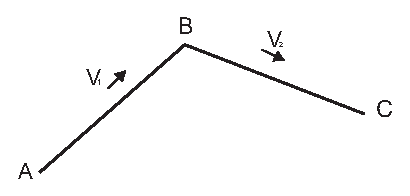
\includegraphics[width=90mm]{3point.eps}
\caption{Два отрезка пути}\label{two_lines}
\end{figure}

По сути своей, нужно равноускоренно провести БПЛА по касательной окружности к данным отрезкам пути. Для этого понадобится узнать точки касания, боковое ускорение, угловую скорость и угол поворота. Каждый летательный аппарат имеет заданное боковое ускорение, обозначим его $a_n$.
Первым делом найдем радиус  по формуле: 
$$r = \frac{V_1^2}{a_n}$$
Затем найдем косинус угла $\alpha$ между отрезками $AB$ И $BC$ по известной формуле:
$$\cos{\alpha} = \frac{\langle V_1,V_2 \rangle}{|V_1||V_2|}$$
Теперь, зная радиус и угол между отрезками пути, можно найти длину $h$~--- расстояние от точки касания до точки стыка двух отрезков пути.

\begin{figure}[ht!]
\centering
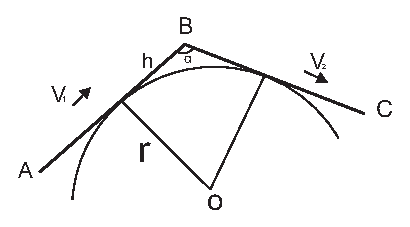
\includegraphics[width=90mm]{3pointCircle.eps}
\caption{Касательная окружность к двум отрезкам пути.}\label{two_lines_and_circle}
\end{figure}
Как видно из рисунка~\ref{two_lines_and_circle}, так как радиус, проведенный в точку касания, перпендикулярен касательной линии, длину $h$ можно найти, вычислив тангенс половинного угла $\alpha$, затем умножив его на радиус $r$. По известной тригонометрический формуле 
$$
  \tg{\frac{\alpha}{2}} := \sqrt{\frac{1-\cos{\alpha}}{1+\cos{\alpha}}}.
$$
Значит 
$$h := r \cdot \sqrt{\frac{1-\cos{\alpha}}{1+\cos{\alpha}}}$$

Теперь можно найти координаты точек касания отступив от точки $B$, на расстояние $h$ вдоль отрезков. Для этого найдем нормированные вектора $a,c$, которые смотрят вдоль  на точки $A,  C $ соответственно: 
\begin{align*}
    &a:=\frac{BA}{|BA|},\\
    &c:=\frac{BC}{|BC|}
\end{align*}
.

Находим точки касания $A',C'$:
\begin{align*}
    &A' := a \cdot h, \\
    &C' := c \cdot h
\end{align*}
\newpage

\begin{figure}[ht!]
\centering
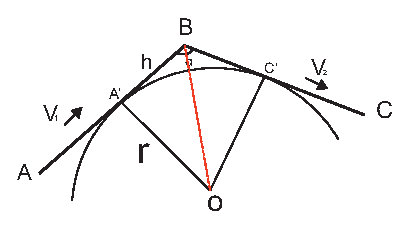
\includegraphics[width=90mm]{tochki_kasania.eps}
\caption{Касательная окружность к двум отрезкам пути.}\label{two_lines_and_circle_2}
\end{figure}

Так как траектория пути находится в трехмерном пространстве, нужно использовать формулу поворота для трехмерного пространства:
\begin{align*}\label{rotation_formula}
        &x' = (\cos{\theta} + n_x^2(1-\cos{\theta}))x + (n_x n_y (1-\cos{\theta}) - n_z\sin{\theta})y + (n_x n_z(1-\cos{\theta}) + n_y \sin{\theta})z \\
        &y' = (n_x n_y (1-\cos{\theta}) - n_z\sin{\theta})x + (\cos{\theta} + n_y^2(1-\cos{\theta}))y + (n_y n_z(1-\cos(\theta)) - n_x\sin{\theta})z\\
        &z' = (n_x n_z(1-\cos{\theta}) + n_y \sin{\theta})x + (n_y n_z(1-\cos(\theta)) - n_x\sin{\theta})y + (\cos{\theta} + n_z^2(1-\cos{\theta}))z
\end{align*}
где $n = (n_x,n_y,n_z)^\text{\textup{T}}$~--- нормированный вектор оси вращения, $\theta$~--- угол, на который нужно повернуть, $r' = (x',y',z')^\text{\textup{T}}$~--- новые координаты точки на окружности,$r=(x,y,z)^\text{\textup{T}}$ - старые координаты. Также, нужно учесть, что поворот в данной формуле происходит вокруг точки начала, то есть нужно будет сдвинуть старые координаты на радиус вектор центр окружности $r_0=(x_0,y_0,z_0)^\text{\textup{T}}$, а затем новые координаты сдвинуть обратно. То есть, формула будет выглядеть следующим образом:
\begin{align*}
        x' &= x_0 + (\cos{\theta} + n_x^2(1-\cos{\theta}))(x-x_0) + (n_x n_y (1-\cos{\theta}) - n_z\sin{\theta})(y - y_0)+{} \\ 
        & + (n_x n_z(1-\cos{\theta}) + n_y \sin{\theta})(z-z_0) \\
        y' &= y_0 + (n_x n_y (1-\cos{\theta}) - n_z\sin{\theta})(x - x_0) + (\cos{\theta} + n_y^2(1-\cos{\theta}))(y - y_0)+{} \\ 
        &+ (n_y n_z(1-\cos(\theta)) - n_x\sin{\theta})(z - z_0)\\
        z' &= z_0 + (n_x n_z(1-\cos{\theta}) + n_y \sin{\theta})(x - x_0) + (n_y n_z(1-\cos(\theta)) - n_x\sin{\theta})(y-y_0) +{} \\&+ (\cos{\theta} + n_z^2(1-\cos{\theta}))(z - z_0)
\end{align*}

Для нахождения вектора оси поворота $n$, нам понадобятся, уже известные, вектора $a$ и $c$, а точнее их векторное произведение, ведь по сути нам нужно найти нормированный вектор, перпендикулярный плоскости, в которой происходит поворот. А мы знаем что вектора $a,c$ лежат в этой плоскости. Находим вектор оси следующим образом:
$$n=\frac{c\times a}{|c\times a|}$$
Также, нужно отметить, что порядок умножения именно такой, ведь это задаст правильную ориентацию поворота.

%??? картинку с осью и углом поворота

%??? возможно стоит написать про то как правильно вычислять скорость
\subsection{Радиоканал}
У каждого ЛА на борту есть радиопередатчик. Раз в определенное время каждый аппарат сообщает свое текущее состояние, на момент вещания, и свой краткосрочный план движения. В текущее состояние входит такая информация как время вещания, имя ЛА, координаты позиции, вектор скорости, модуль скорости. А в краткосрочный план входят 4 будущие позиции маршрута, то есть координаты точек в пространстве и момент времени, когда ЛА будет в ней находится. 

Моменты на которые просчитываются прогнозы зафиксированы. При прохождении первой точки из набора она удаляется из набора и добавляется новая точка после последней и обновленный набор вещается в эфир.

При перестройке маршрута в эфир сообщается новый набор прогнозируемых точек.

Считается, что все бортовые часы БПЛА синхронизированы с достаточной точностью.

Вещание нужно для общения летательных аппаратов между собой, чтобы предотвращать конфликты.

\subsection{Обнаружение конфликтов}
Как уже упоминалось в пункте выше, каждый ЛА сообщает в радио канал свои будущие позиции для определения конфликтных промежутков времени.

Проверка делится на несколько этапов, а именно на фильтрацию по дальности, фильтрацию по сближению и на детальный анализ планов движения

Разберемся как происходит фильтрация тех аппаратов, с которыми точно не может быть конфликта. 
Первой проверкой является проверка расстояния, у каждого ЛА есть радиус фильтрации, если расстояние между аппаратами превышает заданное, то дальнейшее рассмотрение не требуется. 

\begin{figure}[ht!]
    \begin{tikzpicture}[>=latex]
        \draw[thick,dotted] (1,1) circle (2cm); % окружность
        \fill[blue] (1,1) circle (2pt); % центр
        \draw[blue, -]  (1,1) -- node[left=3pt] {$R$}  (1,3) ; % радиу
        \fill[red] (2,3) circle (2pt);
        \fill[red] (2,1.5) circle (2pt);
    \end{tikzpicture}
    \caption{Радиус фильтрации}\label{radius_filter}
\end{figure}

Если же БПЛА находятся на меньшем расстоянии, то переходим к следующей проверке, фильтрации по сближению. Она заключается в том, что считается скалярное произведение по следующей формуле:
$<p_2 - p_1, v_2 - v_1 >,$
где $p_1, p_2$ - точки позиций в пространстве первого и второго судна соответственно, 
$v_1, v_2$ - векторы скорости первого и второго судна соответственно.
\begin{figure}[ht!]
    \begin{tikzpicture}[>=latex]
        \draw[thick,dotted] (1,1) circle (2cm); % окружность
        \fill[blue] (1,1) circle  (2pt); % ла 1
        \fill[red] (2,1.5) circle (2pt); % ла 2

        \coordinate [label=left:$p_1$] (A) at (1,1); % обозн точки ла 1
        \coordinate [label=right:$p_2$] (B) at (2,1.5); % обозн точки ла 2
        \coordinate [label=left:$v_1$] (A1) at (1,2);
        \coordinate [label=right:$v_2$] (B1) at (1.5,2);

        \draw [->] (A) -- (B);

        \draw [->,blue] (A) -- (A1);

        \draw [->,red] (B) -- (B1);

        \draw [->] (A1) -- (B1);
    \end{tikzpicture}
    \caption{Отфильтрованный ЛА}\label{check_scalar_product}
\end{figure}

Если скалярное произведение больше либо равно нуля, значит конфликта нет, если же оно отрицательно, то нужно переходить к вычислению конфликтных промежутков.

Теперь рассмотрим, как происходит анализ планов. Так как, у будущих точек, которые транслируют ЛА, чаще всего имеют разные моменты времени, то требуется провести подготовительные работы, а именно "нормировать" сетку у плановых точек перемещения. Под "нормированием", имеется ввиду добавление вспомогательных точек, в те моменты времени, которых нет в пути, который сообщил ЛА в радиоканал. На всех промежутках, считаем, что БПЛА двигаются равномерно-прямолинейно от начала до конца отрезка движения. Новые точки, вычисляются следущим образом:
\begin{align*}
    &x = x_i^0 + v_i^x(t - t_{i}),\\
    &y = y_i^0 + v_i^y(t - t_{i}),\\
    &z = z_i^0 + v_i^z(t - t_{i}),
\end{align*}
где $i$ --- номер промежутка, $x, y, z$ --- координаты новых точек маршрута, $t_i$ --- время начала рассматриваемого промежутка, $t$ - время вычисляемой точки, $v_i^x,v_i^y,v_i^z$ --- координаты вектора скорости на данном промежутке.

Теперь, когда сетки пути номинированные, можно приступить к анализу. Весь анализ сводится к нахождению временных промежутков конфликта. Для этого нужно пройтись по каждому отрезку движения и проверить, есть ли на нем конфликт в плоскости $OXZ$ и оси $Y$. Под конфликтом имеется ввиду, попадает ли другой ЛА, в радиус защитного объема(ЗО) в горизонтальной плоскости и в высоту защитного объема по вертикальной оси. Каждую точку рассматриваемого отрезка для каждого ЛА можно представить следующим образом:
\begin{align*}
    &x_i(t) = x_0 + v_i^x(t - t_0),\\
    &y_i(t) = y_0 + v_i^y(t - t_0),\\
    &z_i(t) = z_0 + v_i^z(t - t_0)
\end{align*}
, где $i$ --- номер ЛА.

Теперь рассмотрим ситуацию, где у нас всего два ЛА с номерами 1 и 2. Тогда имеем  следующие условия:

\begin{align*}
    ||(x_1(t), z_1(t))^T - (x_2(t), z_2(t))^T|| &\leq R_{30},\\
    |y_1(t) - y_2(t)| &\leq H_{30}\\
\end{align*}

Продолжая раскрывать , получим два квадратных уравнения, решения которых будут являться концы промежутков конфликта.

\newpage
\section{Практическая часть}
Программа была реализована на языке C++, в среде разработки Microsoft Visual Studio. Выбор стал именно таким, так как он обеспечивает нужное быстродействие вычислений и кроссплатформенность. Все графики были сформированы в Gnuplot 6.0. В данный момент в программе реализовано две динамические модели~--- материальная точка и коптер. 

\subsection{Вспомогательные классы и методы}
Для данной работы были написаны вспомогательные классы  и методы для работы с ними такие как:
\begin{itemize}
    \item \texttt{Vector3}~--- класс для удобной работы с трехмерными векторами. По сути своей класс обладает тремя полями $x,y,z$ для определения координат. В нем были реализованы базовые операции над векторами: 
    \begin{itemize}
      \sloppy
        \item \texttt{+}~--- сложения и вычитание векторов
        \item \texttt{*}~--- умножения вектора на скаляр
        \item \texttt{/}~--- деления вектора на скаляр
        \item \texttt{*}~--- умножение вектора на скаляр
        \item \texttt{double scalarProduct(Vector3 v1, Vector3 v2)}~--- скалярное произведение трёхмерных векторов
        \item \texttt{Vector3 crossProduct(Vector3 v1, Vector3 v2)}~--- векторное произведение трёхмерных векторов
  
        \item \texttt{void rotate(Vector3 axis, Vector3 axisPoint, double angle)}~--- операция поворота вектора вокруг заданной оси и точки, через которую проходит это ось, на заданный угол
        \item \texttt{double norm()}~--- подсчет длины вектора
        \item \texttt{Vector3 getNormVector()}~--- получение нормированного вектора из данного
    \end{itemize}
    \item \texttt{Point}~--- структура для описание точки пути, который задает пользователь. Он состоит из полей:
    \begin{itemize}
        \item \texttt{Vector3 position}~--- поле для хранения координат позиции точки
        \item \texttt{double time}~--- момент времени, в который должен оказаться ЛА в заданной позиции
    \end{itemize}
    \item \texttt{TurnData}~--- структура для хранения данных, которые нужно для поворота. Имеет следующею поля:
    \begin{itemize}
        \item \texttt{double angularVelocity}~--- поле для хранения предвычисленного углового ускорения, используется для поворота позиции по окружности
        \item \texttt{Vector3 axisPoint}~--- поле для хранения точки оси поворота
        \item \texttt{double angularVelocity\_0}~--- поле для хранения предвычисленного углового ускорения, используется для вычисления скорости при повороте
        \item \texttt{double angularAcceleration}~--- поле для хранения углового ускорения
        \item \texttt{Vector3 axis}~--- поле для хранения оси поворота
    \end{itemize}
    \item \texttt{PathPointType}~--- класс перечислений, для пометки точек траектории прокладки. Содержит:
        \begin{itemize}
            \item \texttt{DEFAULT}~--- тип для обозначения точки, после которой движение прямолинейное, равномерное.
            \item \texttt{START\_TURN}~--- тип для обозначения точки, после которой начинается маневр поворота 
        \end{itemize}
    \item \texttt{PathPoint}~--- структура для описания точки пути прокладки, является наследником класса \texttt{Point}. Состоит из:
    \begin{itemize}
        \item \texttt{Vector3 position}~--- поле для хранения координат позиции точки
        \item \texttt{double time}~--- момент времени, в который должен оказаться ЛА в заданной позиции
        \item \texttt{PointType type}~--- поле для типа точки
        \item  \texttt{TurnData turnData}~--- поле для данные поворота. 
    \end{itemize}
    \item \texttt{Path}~--- класс для описания пути прокладки. Имеет следующие методы и поля:
    \begin{itemize}
        \item \texttt{vector<PathPoint> path}~--- приватное поле для хранения вектора, состоящего из точек типа. \texttt{PathPoint}.
        \item \texttt{PathPoint getPointForIndex(int ind)}~--- метод для получения точки пути по индексу.
        \item \texttt{void addNewPoint(PathPoint p)}~--- метод для добавления точки в траекторию прокладки.
    \end{itemize}
    \item \texttt{FVState}~--- структура для передачи состояния и короткого плана в радиоканал.  
    \begin{itemize}
        \item \texttt{Plane plane}~--- поле для записи текущего состояния
        \item \texttt{vector<Point>}~--- поле для записи плана движения на следующие 4 точки пути.
    \end{itemize}
    \item \texttt{AEtherInfo}~--- класс, который служит радиоканалом для всех ЛА.  
    \begin{itemize}
        \item \texttt{map<string,FVState> states}~---  поле куда ЛА записывают свои данные.
        \item \texttt{void broadcastState(const Plane\& plane)}~--- метод, принимающий текущее состояние ЛА и записывает в соответствующее поле радиоканала.
        \item \texttt{void broadcastPlan(const string\& name,\\ const vector<Point>\& shortPlan)}~--- метод, который принимает имя и короткий маршрутный план и записывает их соответствующее поле радиоканала.
    \end{itemize}
    \item \texttt{GlobalSituation}~--- класс для хранения глобального состояния всего моделирования.  
    \begin{itemize}
        \item \texttt{vector<FV*> FVs}~---  поле для хранения ссылок на каждый ЛА, участвующий в моделировании.
        \item \texttt{AEtherInfo aetherInfo}~--- поле для хранения радиоканала моделирования.
    \end{itemize}
    \item \texttt{DataParser.h}~--- файл с методами для подгрузки входных данных по ЛА.   
    \begin{itemize}
        \item \texttt{void ParseSolveDataFromJSON(string json\_name, double\& time\_step,\\ double\& integration\_h, int\& solve\_part\_count)}~--- метод для сбора данных для вычислений из файла.
        \item \texttt{void ParsePathFromJSON(const json\& path\_data, vector<Point>\& path);}~--- метод для сбора данных пути ЛА.
        \item \texttt{void ParseFVToList(string json\_name, GlobalSituation\& gs);}~--- метод для сбора данных об ЛА из файла в список.
    \end{itemize}
    \item \texttt{check}~--- класс предназначенный для сравнения по точности.   
    \begin{itemize}
        \item \texttt{static bool EQ(double value\_1, double value\_2);}~---  метод сравнения равенства по точности 
        \item \texttt{static bool NOTEQ(double value\_1, double value\_2);}~--- метод сравнения не равенства по точности
        \item \texttt{static bool RE(double value\_1, double value\_2);}~--- метод сравнения больше по точности
        \item \texttt{static bool REQ(double value\_1, double value\_2);}~--- метод сравнения больше меньше по точности
        \item \texttt{static bool LE(double value\_1, double value\_2);}~--- метод сравнения меньше по точности
        \item \texttt{static bool LEQ(double value\_1, double value\_2);}~--- метод сравнения меньше равно по точности
    \end{itemize}
    \item \texttt{Parameters}~--- структура для параметров, которые будут записаны в выходном файле, предназначенные для описания ЛА.
    \begin{itemize}
        \item \texttt{string name;}~--- поле для ранения имени ЛА
        \item \texttt{string type;}~--- поле для хранения типа ЛА.
        \item \texttt{vector<Point> plan;}~--- поле для планового пути движения ЛА.
    \end{itemize}
    \item \texttt{DynamicData}~--- структура для динамичных данных, которые будут записаны в выходной файл. 
    \begin{itemize}
        \item \texttt{double t}~--- поле для хранения времени 
        \item \texttt{double x}~--- поле для хранения координаты x
        \item \texttt{double y}~--- поле для хранения координаты y
        \item \texttt{double z}~--- поле для хранения координаты z 
    \end{itemize}
    \item \texttt{BroadcastData}~--- структура для данных, которые транслируются каждым ЛА в радио канал
    \begin{itemize}
        \item \texttt{double t}~--- поле для хранения времени 
        \item \texttt{double x}~--- поле для хранения координаты x
        \item \texttt{double y}~--- поле для хранения координаты y
        \item \texttt{double z}~--- поле для хранения координаты z
        \item \texttt{string type;}~--- поле для типа транслируемых данных
       \item \texttt{vector<Point> plan;}~--- поле для короткого плана
    \end{itemize}
    \item \texttt{OutputFV}~--- структура для описания данных вывода в файл описывающих ЛА
    \begin{itemize}
        \item \texttt{Parameters parameters;}~--- поле для параметров
        \item \texttt{vector<DynamicData> dynamic\_data;}~--- поле для списка динамичских данных
        \item \texttt{vector<BroadcastData> broadcasts;}~--- поле для списка тарнслируемых данных
    \end{itemize}
    \item \texttt{OutputJsonData}~--- структура для описания выходных данных
    \begin{itemize}
        \item \texttt{string version}~--- поле для версии файла
        \item \texttt{vector<OutputFV> FVs}~--- поле для списка выходных данных по каждому ЛА.
    \end{itemize}
    \item \texttt{void writeJsonData(const string\& file\_name,\\ const OutputJsonData\& output\_json\_data)}~--- метод для записи выходных данных в формате json.
     \item \texttt{Modeler}~--- класс для инкапсуляции всего процесса моделирования.
    \begin{itemize}
        \item \texttt{void startModeling()}~---  метод для запуска процесса  моделирования.
        \item \texttt{double solve\_time}~--- поле для хранения промежутка времени, на которое нужно делать следующее вычисление.
        \item \texttt{double integral\_h}~--- поле для хранения шага интегрирования.
        \item \texttt{int solve\_part\_count}~--- поле для хранения количества вычислений.
        \item \texttt{double start\_time}~--- поле для хранения момента времени начала вычислений.
        \item \texttt{double end\_time}~--- поле для хранения момента времени конца вычислений.
        \item \texttt{GlobalSituation globalSituation}~--- поле для хранения глобальных данных моделирования.
    \end{itemize}
    \item \texttt{void mergeShortPlans(const vector<Point>\& arr1, const vector<Point>\& arr2,
	vector<Point>\& res1, vector<Point>\& res2)}~--- метод нормирования сеток трнаслируемых планов движения в радио канал.
\end{itemize}
\subsection{Входные данные}
Входные данные программы представляют собой json файл следующей структуры:
\begin{verbatim}
{
  "timeStep": 1,
  "solve_part_count": 10,
  "AirCraftList": [
    {
      "type": "MaterialPoint",
      "fv_id": "first",
      "parameters": {
        "v_x": 0,
        "v_y": 0,
        "v_z": 0,
        "maxAcceleration": 1,
        "k_xz": -1,
        "k_y": -1,
        "broadcastStep": 2,
        "radiusFilter": 5,
        "heightWarn": 2,
        "radiusWarn": 3
      },
      "path": [
        {
          "time": 0,
          "x": 0,
          "y": 0,
          "z": 0
        },
        ...
      ]
    }
\end{verbatim}
\begin{itemize}
    \item \texttt{timeStep}~--- шаг вывода вычислений
    \item \texttt{solve\_part\_count}~--- кол-во вычислений итегрирования
    \item \texttt{AirCraftList}~--- список описаний ЛА.
    \begin{itemize}
        \item \texttt{type}~--- тип ЛА.
        \item \texttt{fv\_id}~---  id ЛА.
        \item \texttt{parameters}~--- параеметры ЛА.
        \begin{itemize}
            \item  \texttt{v\_x}~--- координата вектора скорости по оси X
            \item  \texttt{v\_y}~--- координата вектора скорости по оси Y
            \item  \texttt{v\_z}~--- координата вектора скорости по оси z
            \item \texttt{maxAcceleration}~--- максимальное ускорение
            \item\texttt{k\_xz}~--- коэффициент управления по xz
            \item\texttt{k\_y}~--- коэффициент управления по y
            \item\texttt{broadcastStep}~---шаг трансляции
            \item\texttt{radiusFilter}~--- радиус фильтрации
            \item\texttt{heightWarn}~--- высота защитного объема 
            \item\texttt{radiusWarn}~--- радиус защитного объема
        \end{itemize}
        \item \texttt{path}~--- список точек пути
        \begin{itemize}
            \item \texttt{time}~--- момоент времени
            \item \texttt{x}~--- координата x
            \item \texttt{y}~--- координата y
            \item\texttt{z}~--- координата z
        \end{itemize}
    \end{itemize}
\end{itemize}

\subsection{Выходные данные}
Выходные данные программы представляют собой json файл следующей структуры:
\begin{verbatim}
{FVs: [
  {
    parameters : { 
        name: ...,
        plane: [...],
        type: ...
    },
    dynamic_data : { 
        {
            t: ...,
            x: ...,
            y: ...,
            z: ...,
        },
        ...
    },
    broadcasts : [
        {
            "plan": [...],
            "t": ...,
            "type": ...,
            "x": ...,
            "y": ...,
            "z": ...,
        },
        ...
    ]
  },
  { ... }
]}
\end{verbatim}
\begin{itemize}
    \item \texttt{parameters}~--- параеметры ЛА.
    \begin{itemize}
            \item  \texttt{name}~--- имя ЛА.
            \item  \texttt{plane}~--- плановый путь ЛА.
            \item  \texttt{type}~--- тип ЛА.
    \end{itemize}
    \item \texttt{dynamicData}~--- список точек движения ЛА вычисленных на каждой итерации
    \begin{itemize}
            \item \texttt{t}~--- момоент времени
            \item \texttt{x}~--- координата x
            \item \texttt{y}~--- координата y
            \item\texttt{z}~--- координата z
    \end{itemize}
    \item \texttt{broadcasts}~--- список сообщений ЛА в радиоканал.
    \begin{itemize}
            \item  \texttt{plane}~--- короткий плановый путь, на следующие 4 точки.
            \item  \texttt{t}~--- время вещания.
            \item  \texttt{type}~--- тип вещания, либо позиции либо короткого плана.
            \item  \texttt{x}~--- координата позиции x.
            \item  \texttt{y}~--- координата позиции y.
            \item  \texttt{z}~--- координата позиции z.
    \end{itemize}
\end{itemize}
\subsection{Реализация динамических моделей}
Для реализации динамических моделей был создан базовый абстрактный класс FV. Он определяет базовые свойства присущие каждой модели движения, такие как:
\begin{itemize}
    \item     \texttt{virtual void next(double h, double end\_time) = 0}~--- виртуальная функция, которая служит для вычисления следующего состояния БПЛА с шагом $h$ до момента $end\_time$.
    \item \texttt{virtual void setPath(vector<Point> path)}~--- виртуальная функция, которая служит для вычисления прокладки пути. По умолчанию вычисляется по схеме прокладки с упреждением поворота.
    \item \texttt{void doBroadcast()}~--- метод для трансляции данных в радио канал.
    \item \texttt{void checkConflict()} -- метод для проверки конфликтов.
    \item \texttt{vector<Point> getBasePath()}~--- возвращает базовый путь, введенный пользователем.
    \item \texttt{Path getDynamicPath()}~--- возвращает построенный путь прокладки при задании пути.
    \item \texttt{vector<Point> basePath}~--- поле для хранения базового пути, который вводит пользователь.
    \item \texttt{Path turnPath}~--- поле для хранения, пути прокладки, заданной с помощью метода  \texttt{setPath}.
    \item \texttt{Path dynamicPath}~--- поле для хранения динамически изменяемого пути  \texttt{setPath}.
    \item \texttt{virtual double solveTurnRadius(const Vector3\& v1, const Vector3\& v2)}~---\\ метод,  принимающий две скорости ЛА на соседних промежутках. Вычисляет радиус поворота.
    \item \texttt{double time}~--- поле для хранения времени текущего состояния БПЛА
     \item \texttt{double broadсastStep}~--- поле, в котором записан шаг вещания.
      \item \texttt{double nextBroadcastInstant}~--- поле для следующего момента времени вещания.
    \item \texttt{GlobalSituation\* globalSituation}~--- поле для хранения указателя на глобальное состояние.
\end{itemize}
Далее рассмотрим подробнее конкретные реализации динамических моделей~--- материальной точки и коптера, которые являются наследниками класса \texttt{FV}

\subsubsection{Материальная точка}
Класс материальной точки \texttt{MaterialPoint} является публичным наследником класса \texttt{FV}. А значит обладает всеми уже ранее описанными методами и полями, но также имеет и собственные. А именно:
\begin{itemize}
    \item \texttt{string getName()}~--- метод возвращающий имя БПЛА.
    \item \texttt{int32\_t getType()}~--- метод метод возвращающий тип БПЛА, у материальной точки 0.
    
    \item \texttt{Vector3 acceleration}~--- поле которое хранит ускорение в текущем состоянии.
    \item \texttt{Vector3 wishPosition}~--- поле хранящее желаемую позицию, вычисленную в методе \texttt{computeWishData}.
    \item \texttt{Vector3 wishVelocity}~--- поле хранящее желаемую скорость, вычисленную в методе \texttt{computeWishData}.
    \item \texttt{string name}~--- поле, содержащее имя БПЛА.
    \item \texttt{int32\_t type}~--- поле, хранящее тип БПЛА.

    \item\texttt{Vector3* curPosition}~--- поле хранящее указатель на текущую позицию БПЛА.
    \item\texttt{Vector3* newPosition}~--- поле хранящее указатель на новую позицию, вычисленную в методе \texttt{next}.
    \item\texttt{Vector3* curVelocity}~--- поле хранящее указатель на текущую скорость БПЛА.
    \item\texttt{Vector3* newVelocity} поле хранящее указатель на новую скорость, вычисленную в методе \texttt{next}
    \item\texttt{double k\_v}~--- поле хранящее значение коэффициента вклада позиции на управление.
    \item\texttt{double k\_x}~--- поле хранящее значение коэффициента вклада скорости на управление.
    \item\texttt{double maxAcceleration}~--- поле хранящее значение максимального ускорения.\textbf{}
    
    \item\texttt{void computeWishData(double time\_solve)}~--- метод предназначенный для вычисления желаемой позиции и желаемой скорости в момент времени \texttt{time\_solve}
\end{itemize}

\subsubsection{Коптер}
Класс коптер \texttt{Copter}, также как и материальная точка является публичным наследником класса \texttt{FV}. А значит обладает всеми уже ранее описанными методами и полями, но также имеет и собственные, почти во всем перекликается с материальной точкой, но также имеет собственные особенности:
\begin{itemize}
    \item \texttt{double inertialXZ}~--- поле для хранения коэффициента инерции в плоскости $OXZ$. 
    \item \texttt{double inertialY}~--- поле для хранения коэффициента инерции по оси $OY$.
\end{itemize}
\subsection{Вычисление <<штурманской>> прокладки}

\subsubsection{Разметка траектории}
Разберем весь процесс вычисления, того как должен двигаться БПЛА. 
Начнем с метода \texttt{setPath} прописанного в базовом классе \texttt{FV}.
Данный метод, как упоминалось ранее, принимает вектор из точек траектории пользователя, а затем пробегает по всем его точкам, проверяя отрезки на наличии поворотов.
Если поворот нужен, то вместо точек стыка двух отрезок заменяют две точки, к которые являются касательными. Первая точка касания помечается типом \texttt{PointPathType::START\_TURN} и для нее вычисляются все данные для поворота, указанные в структуре \texttt{TurnData}. После данного процесса полученный путь сохраняется в поле \texttt{Path dynamicPath}.

%???? Нужна ли вставка с кодом ????
\subsubsection{Вычисление прокладки}
Метод \texttt{computeWishData} вычисляет \texttt{wishPosition, wishVelocity} желаемые позицию и скорость соответственно по моменту времени. Данный метод идентичен как в классе \texttt{MaterialPoint}, так и в классе \texttt{Copter}. В самом начале бинарным поиском происходит нахождение соответствующего отрезка в \texttt{Path dynamicPath}. Затем, относительного типа точки пути вычисляется желаемая скорость, а после желаемая позиция. Если точка имеет тип \texttt{DEFAULT}, то это значит что нужно двигаться равномерно, прямолинейно до следующей точки, если же тип \texttt{START\_TURN}, то используя данные для поворота из соответствующего поля структуры, вычисляем скорость, находя касательный к окружности вектор, с помощью векторного произведения вектора угловой скорости и радиус вектора с началом в точке в центре окружности и концом в точке позиции БПЛА. Для вычисления новой позиции на окружности, последняя позиция двигается с помощью метода \texttt{rotate}, в котором реализована формула поворота.

\subsubsection{Вычисление движения}
Теперь перейдем к методу \texttt{next} для материальной точки. В данном методе происходит вычисление действительной позиции и скорости БПЛА посредством численного интегрирования. Для интегрирования используется метод Эйлера на левый край, где за производную управление берется регулятор, построенный в соответствующем пункте теоретической части. Регулятор используется один и тот же как для материальной точки:
\begin{verbatim}
for (int i = 0; i < 3; i++) {
    double x = (*curPosition)[i];
    double v = (*curVelocity)[i];
    (*newPosition)[i] = x + h * v;
    (*newVelocity)[i] = v + h * k_x * (x -  wishPosition[i] 
                              + k_v * (v - wishVelocity[i]));
    acceleration[i] = k_x * (x - wishPosition[i]) 
                    + k_v * (v - wishVelocity[i]);
}
\end{verbatim}
так и для коптера:
\begin{verbatim}
double x = (*curPosition)[0];
double v = (*curVelocity)[0];
(*newPosition)[0] = x + h * v;
(*newVelocity)[0] = v + h * 
        ((k_v * wishVelocity.x + k_x * wishPosition.x) - v) / inertialXZ;
x = (*curPosition)[1];
v = (*curVelocity)[1];

(*newPosition)[1] = x + h * v;
(*newVelocity)[1] = v + h * 
        ((k_v * wishVelocity.y + k_x * wishPosition.x) - v) / inertialY;

x = (*curPosition)[2];
v = (*curVelocity)[2];

(*newPosition)[2] = x + h * v;
(*newVelocity)[2] = v + h * 
        ((k_v * wishVelocity.z + k_x * wishPosition.x) - v) / inertialXZ;
\end{verbatim}
\subsection{Результаты}

В данном пункте пошагово пройдемся по этапам вычисления. Пусть пользователь задал такой маршрут состоящий из 4 точек: 
\begin{itemize}
    \item $(r_1,t_1) = ((0,0,0),0)$~--- точка для нулевого момента времени,
    \item $(r_2,t_2) = ((10,0,0),10)$~--- точка для 10 секунды,
    \item $(r_3,t_3) = ((10,0,-5),20)$~--- точка для 20 секунды,
    \item $(r_3,t_3) = ((10,0,-15),30)$~--- точка для 30 секунды
\end{itemize}

\begin{figure}[ht!]
\centering
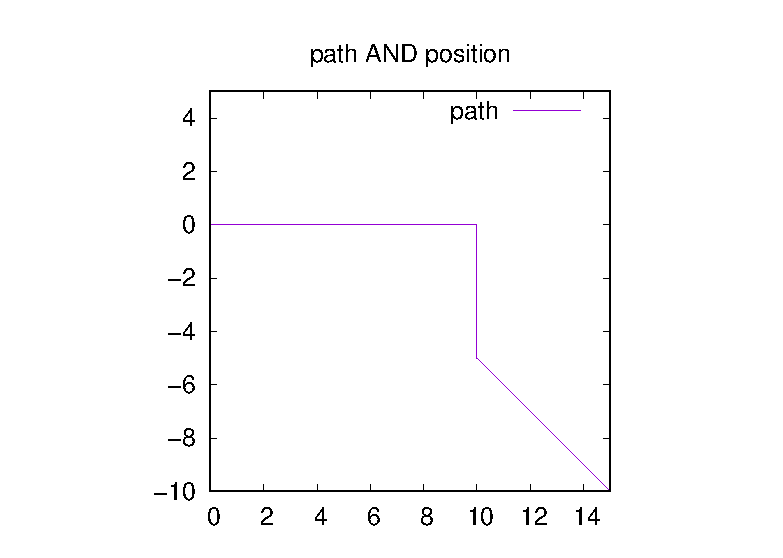
\includegraphics[width=90mm]{default_path.eps}
\caption{ Путь пользователя}\label{user_path}
\end{figure}

Продемонстрирую поведение материальной точки стоящей в нулевой момент времени в точке$(0,0,0)$, с начальной скорость $(0,0,0)$ если использовать <<Наивную>> прокладку. Пусть коэффициенты вклада в управление для позиции и скорости соответственно $k_x = -1$ =,  $k_v = -1$, 

\begin{figure}[H]
\centering
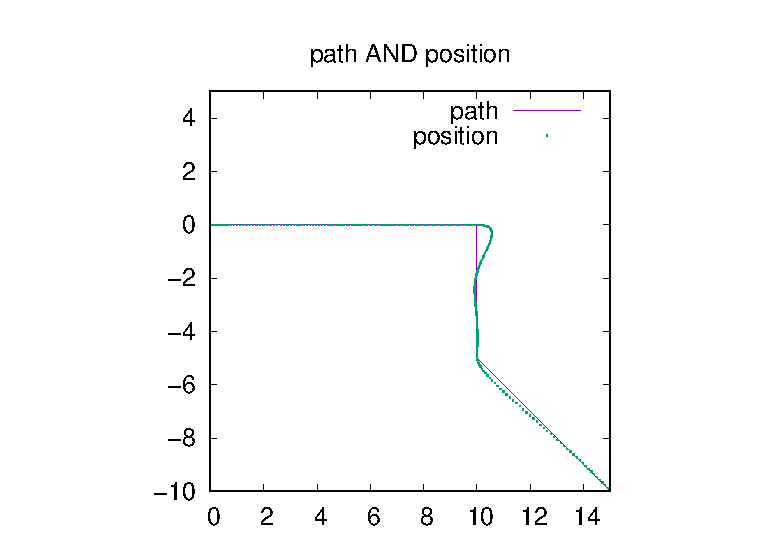
\includegraphics[width=90mm]{default_path_not_procladka.eps}
\caption{ Путь пользователя}\label{not_prokladka}
\end{figure}

Как видно по зеленой линии, летательный аппарат не успевает изменить скорость на повороте.
Теперь построим прокладку с упреждение поворота:

\begin{figure}[ht!]
\centering
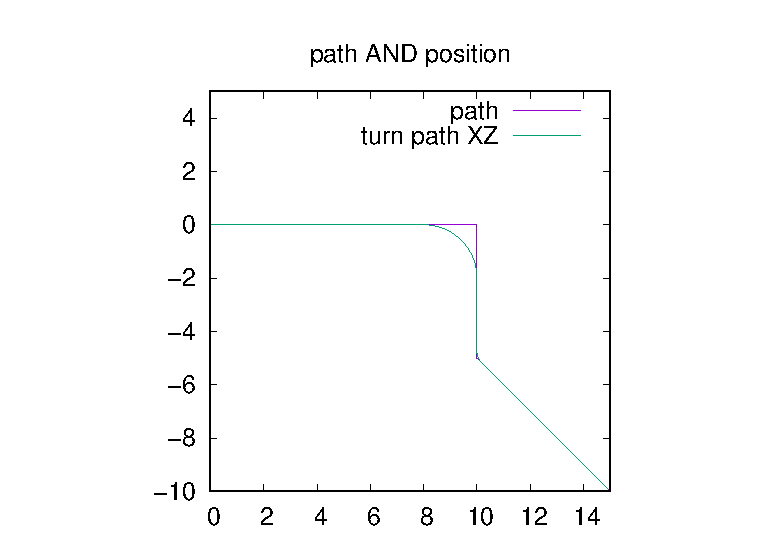
\includegraphics[width=90mm]{default_path_prokladka.eps}
\caption{ Путь пользователя и прокладка}\label{prokladka}
\end{figure}

Посмотрим как будет себя вести БПЛА, нацелившийся на прокладку: 

\begin{figure}[ht!]
\centering
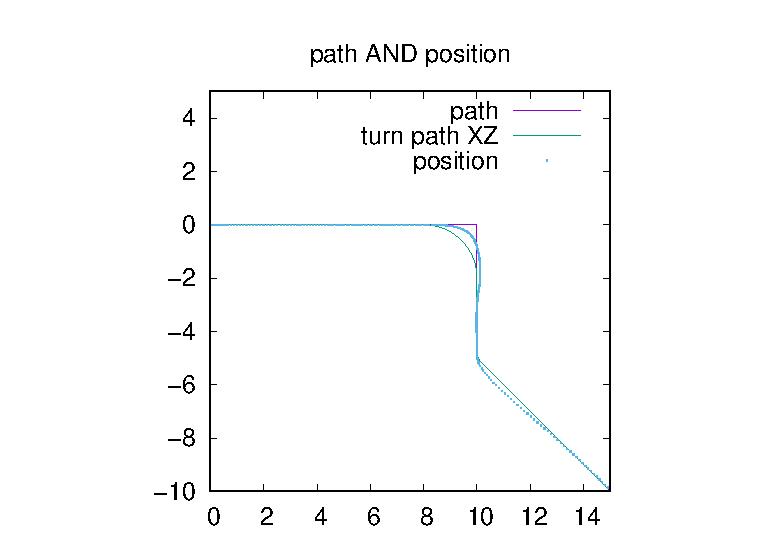
\includegraphics[width=90mm]{default_path_prokladka_position.eps}
\caption{ Путь пользователя}\label{user_path_position}
\end{figure}

Как видно, результат стал намного лучше. Более лучше результата можно добиться подбором коэффициентов $k_x$ и $k_v$, уменьшая или увеличивая вклад желаемых позиции и скорости.

\newpage
\addcontentsline{toc}{section}{Заключение}
\section*{Заключение}
В работе описано построение процедур моделирования движения летательного аппарата вдоль маршрутов, представляющих собой ломаную линию с заданными моментами прибытия ЛА в точки излома. Движение ЛА описывается известных дифференциальных соотношений, включающих управляющие воздействия. Проход точек излома осуществляется прицеливанием постпредством пропорционального регулятора на точку, движущуюся по той или иной штурманской прокладке.    
\newpage
\addcontentsline{toc}{section}{Список литературы}
\begin{thebibliography}{99}
\bibitem{cppSHILD}
Шилдт Герберт C++ базовый курс  [Электронный ресурс]:
Белорусский государственный университет информатики и радиоэлектроники~--- Режим доступа: \url{https://www.bsuir.by/m/12_119786_1_98220.pdf}
(дата обращения: 01.12.2023)

\bibitem{MSC} 
Документация по Microsoft C++, C и ассемблеру [Электронный ресурс]:-- Режим доступа:
\url{https://learn.microsoft.com/ru-ru/cpp/?view=msvc-170} (дата обращения: 01.12.2023).

\bibitem{bib:GOST} ГОСТ 20058-80. Динамика летательных аппаратов в атмосфере. Термины, определения и обозначения.~--- М.:~Госстандарт, 1980.

\end{thebibliography}

\label{LastPage}

\end{document}
